\chapter{Modellierungswerkzeuge}\label{sec:chapter4}
Dieses Kapitel stellt die in dieser Arbeit für die Prozessmodellierung benutzten Modellierungswerkzeuge vor. Nach einer kurzen allgemeinen Einführung in Modellierungswerkzeuge, wird das Modellierungswerkzeug Signavio beschrieben, welches zur imperativen Modellierung von Prozessen mit BPMN in dieser Arbeit herangezogen wird. Anschließend erfolgt eine Einführung in das Modellierungswerkzeug Declare, mit welchem die deklarativen Prozessmodelle in der Prozessmodellierungssprache ConDec in der vorliegenden Arbeit erstellt werden. 

\section{Modellierungswerkzeuge}\label{sec:chapter4:Modellierungswerkzeuge}
Ein Modellierungswerkzeug ist ein Softwaresystem, mit dessen Hilfe sich Prozessmodelle erstellen, ausführen und monitoren lassen. Teilweise bietet ein Modellierungswerkzeug noch weitere Funktionen wie z.B. Simulationen und die Analyse von Prozessmodellen an. Die Ausführung der Prozessschritte kann hierbei durch die jeweilige Person, welche für die Aktivität zuständig ist, ausgeführt werden. Für die Prozessmodellierung in der vorliegenden Arbeit kommt das Modellierungswerkzeug Signavio für die imperative Modellierung mit BPMN und Declare für die deklarative Modellierung mit ConDec zum Einsatz. Diese beiden Modellierungswerkzeuge werden nachfolgend vorgestellt \cite{gadatsch2012}.

\subsection{Signavio}

Bei Signavio handelt es sich um ein webbasiertes Prozessmodellierungstool, welches auch das kollaborative Modellieren von Prozessen mit den Modellierungsstandards BPMN und EPC zulässt. Der Vorteil von Signavio besteht darin, dass es nicht auf dem Rechner installiert werden muss, sondern direkt im Web-Browser ausgeführt werden kann. Die Prozessmodelle werden in einem zentralen Repository gespeichert und sind für die Benutzer entsprechend ihren Zugriffsrechten aufrufbar. Prozessmodelle besitzen alle eine eigene eindeutige URL und können über diese im Web-Browser aufgerufen werden. Hierbei wird auch gleich das Modellierungswerkzeug Signavio mitgeladen und kann somit im Web-Browser ausgeführt werden \cite{quteprints}. \newline
Abbildung \ref{fig:Signavio} zeigt den \textit{Signavio Process Editor}.

\begin{figure}[H]
\begin{center}
  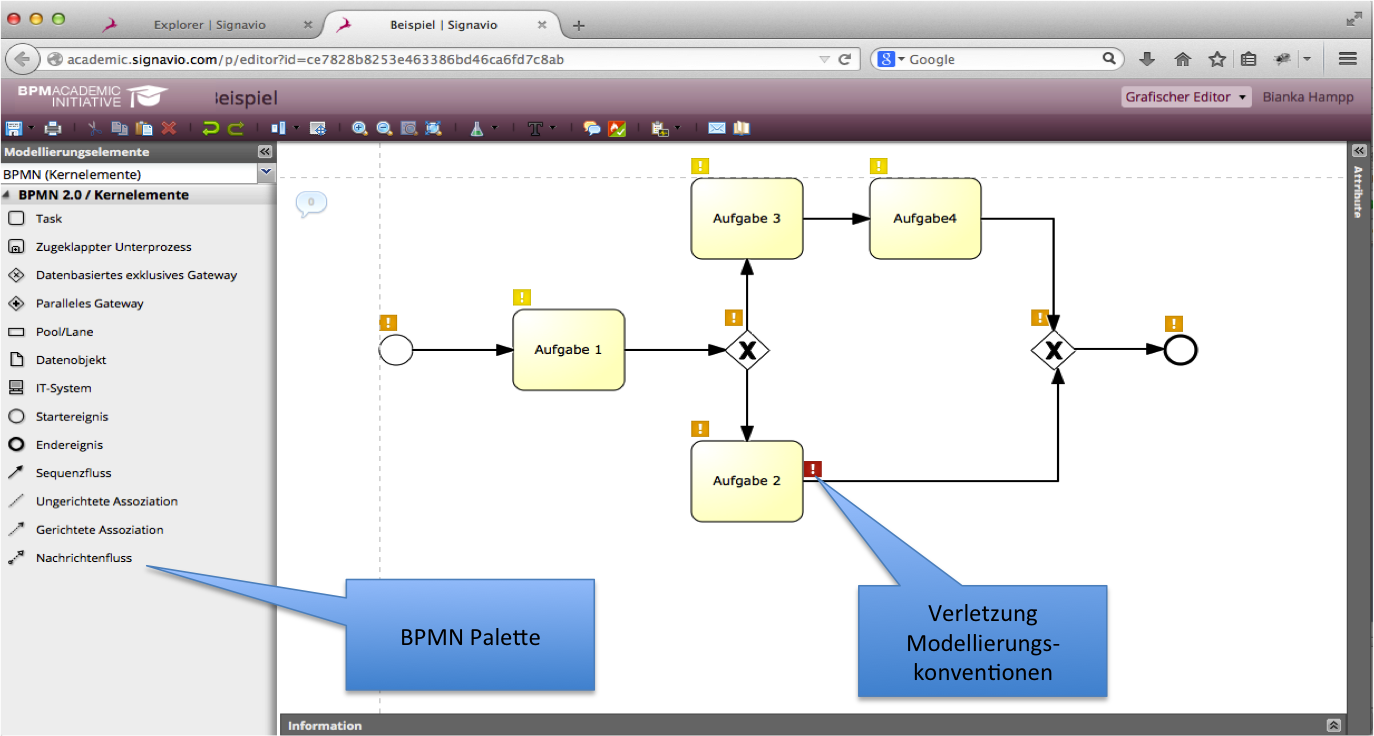
\includegraphics[scale=0.6]{Signavio} %pdf, jpg, png...
  \caption{Siganvio Process Editor (Screenshot Siganvio)}
  \label{fig:Signavio}
\end{center}
\end{figure} 

Links ist die BPMN Palette zu sehen. Die einzelnen Elemente können per \textit{Drag and Drop} in das Arbeitsdokument gezogen werden. Signavio verfügt über Modellierungskonventionen. Mit diesen ist es  möglich, das Modell auf die Einhaltung von Modellierungsrichtlinien, wie z.B. Notationsumfang, Benennung, Prozessstruktur und Diagrammlayout zu überprüfen. Die Modelle können alle als PDF exportiert werden. \newline
In Abbildung \ref{fig:Simulation} ist die Simulations-Sicht von Signavio zu sehen. Hier kann der Benutzer den Prozessablauf simulieren. Dies kann einerseits mit Benutzerinteraktion Schritt für Schritt erfolgen oder auch im Ganzen durch den Simulator gesteuert werden, wobei XOR-Verzweigungen nach wie vor vom Benutzer ausgewählt werden müssen.
\begin{figure}[H]
\begin{center}
  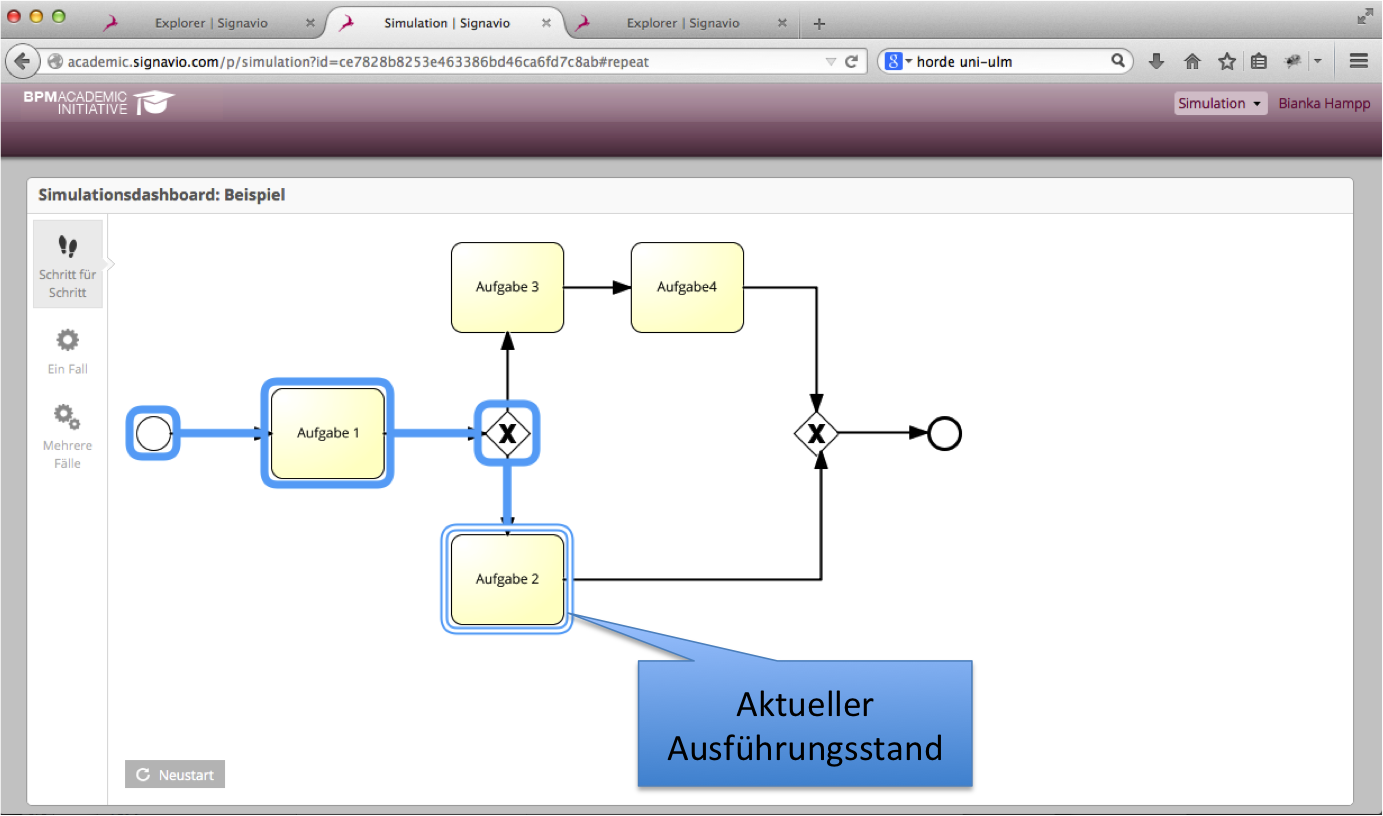
\includegraphics[scale=0.6]{Simulation} %pdf, jpg, png...
  \caption{Siganvio Simulation (Screenshot Signavio)}
  \label{fig:Simulation}
\end{center}
\end{figure} 



\subsection{Declare}

Declare wurde als Constraint-basiertes Workflow-Management-System entwickelt. Es wird für die Entwicklung von Prozessmodellen, welche auf deklarativen Sprachen basieren, benutzt. Declare bietet die folgenden Funktionen an:
\begin {itemize}
\item Modellentwicklung
\item Modellüberprüfung (Suche nach Fehlern in Modellen)
\item automatisierte Modellausführung
\item wechselnde Modelle zur Laufzeit
\item Analyse der bereits durchgeführten Prozesse
\item Prozess Dekomposition
\end {itemize}

Abbildung \ref{fig:Declare} zeigt die Systemarchitektur von Declare.

\begin{figure}[H]
\begin{center}
  \includegraphics[scale=0.8]{Declare} %pdf, jpg, png...
  \caption{Declare Systemarchitektur nach \cite{pesic2007declare}}
  \label{fig:Declare}
\end{center}
\end{figure} 

Hieraus wird ersichtlich, dass \textit{Declare} mit den beiden Systemen \textit{YAWL} und \textit{ProM} kooperiert. Bei \textit{YAWL} handelt es sich hierbei um ein Workflow-Management System, welches auf strukturierte Workflows spezialisiert ist. Dies wirkt sich auf die Zusammenarbeit mit \textit{Declare} in der Art aus, dass die strukturierten Teile des Prozesses von \textit{YAWL} abgehandelt werden, während die unstrukturierten Teile von \textit{Declare} übernommen werden. Bei \textit{ProM} handelt es sich um ein Prozess-Mining-Tool. Hier werden bereits ausgeführte Prozesse von \textit{Declare} analysiert und darauf aufbauend werden dem Nutzer während der Prozessausführung Empfehlungen gegeben \cite{pesic2007declare}. \newline
Weiterhin besteht \textit{Declare} selbst aus drei Komponenten \textit{Framework}, \textit{Designer} und \textit{Worklist}.  Beim \textit{Designer} handelt es sich um ein Modellierungstool, welches für Systemeinstellungen und die Prozessmodell-Entwicklung verwendet wird (Abbildung \ref{fig:Designer}). Das \textit{Framework} ist für das Prozess-Enactment zuständig. Außerdem übernimmt es die Kommunikation mit \textit{YAWL} und \textit{ProM} und das Ändern der Prozessmodelle zur Laufzeit (Abbildung \ref{fig:Framework}). Die Prozessausführung wird von \textit{Worklist} durchgeführt. Hier können die Nutzer ihre zuvor erstellten Prozesse ausführen und können die von \textit{ProM} erstellten Empfehlungen sehen (Abbildung \ref{fig:Worklist}). Alle Modelle können als Bilddateien exportiert werden.



\begin{figure}[H]
\begin{center}
  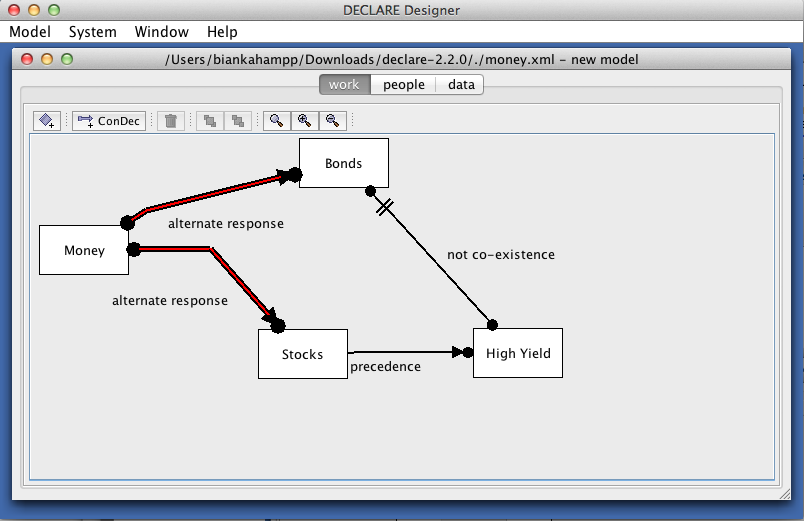
\includegraphics[scale=0.4]{Designer} %pdf, jpg, png...
  \caption{Declare Designer (Screenshot aus Declare)}
  \label{fig:Designer}
\end{center}
\end{figure} 


\begin{figure}[H]
\begin{center}
  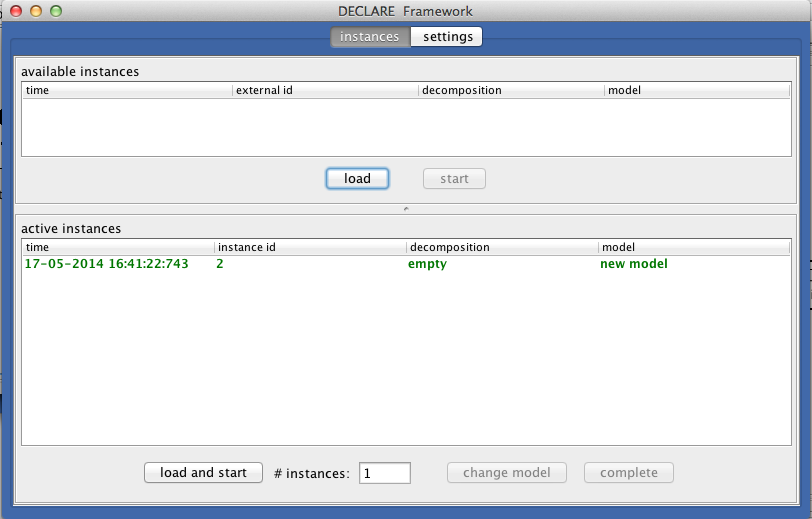
\includegraphics[scale=0.4]{Framework} %pdf, jpg, png...
  \caption{Declare Framework (Screenshot aus Declare)}
  \label{fig:Framework}
\end{center}
\end{figure} 

\begin{figure}[H]
\begin{center}
  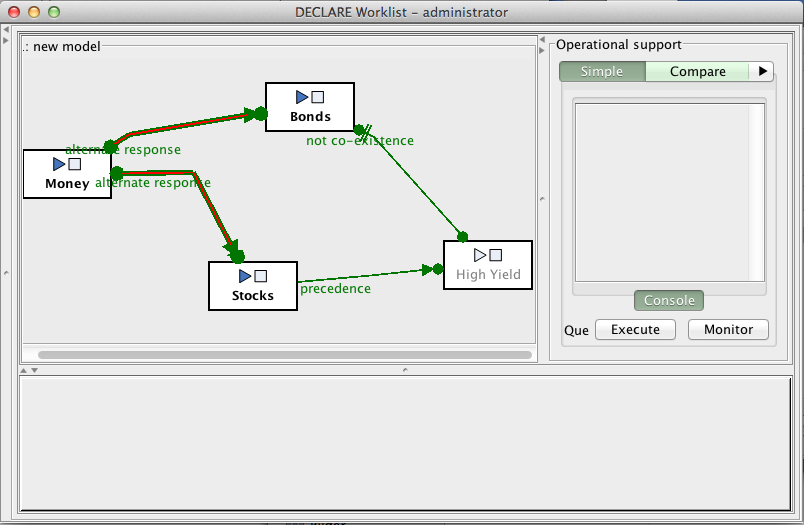
\includegraphics[scale=0.4]{Worklist} %pdf, jpg, png...
  \caption{Declare Worklist (Screenshot aus Declare)}
  \label{fig:Worklist}
\end{center}
\end{figure} 




